\chapter{Weyl semimetals}\label{chap:WSM}

%TODO Intro

{\color{blue}
\begin{itemize}
	\item Give a very brief few-sentence overview of the history behind Weyl fermions (Weyl 1929) and accidental band crossings (Herring 1937) etc.\ here, so the physics section can focus on modern descriptions straight away
	
	\item Credit review papers in introduction
	
	\item This chapter contains no new results, its purpose is to provide the necessary background to our results in Chapter~\ref{chap:non-orientable}.
	
	\item Section~\ref{sec:semimetal-physics} reviews physical aspects of WSM, Section~\ref{sec:semimetal-topology} goes into the topological details.
\end{itemize}
}

\section{Physical aspects}\label{sec:semimetal-physics}

The concept of Weyl semimetals arises naturally when studying how different energy bands interact in three-dimensional solids. Whereas one and two-dimensional materials are generally gapped unless additional symmetries force the bands to touch, the situation is different in three dimensions. In this context, so-called \emph{accidental band crossings} are expected based on geometric arguments.

Accidental crossings can be understood by studying how any two of the energy bands interact. In most physically relevant scenarios these will be the valence and conduction band, since these determine the conductive properties of a material. Recall that the generic Hermitian two-band Hamiltonian can be written as
\begin{equation*}
	\Hc(\k) = h_0(\k)\Id + \h(\k)\cdot\bm{\upsigma},
\end{equation*}
where $\k$ lives in the three-dimensional Brillouin torus $\T^3$ in this case. The eigenvalues of this Hamiltonian are
\begin{equation*}
	E(\k) = h_0(\k) \pm \abs{\h(\k)},
\end{equation*}
so that the gap between the two bands closes exactly when $\h(\k) = 0$. That is, band crossings occur at the simultaneous zeroes of three functions $h_i$ for $i\in\set{1,2,3}$, all depending on three momentum degrees of freedom. Such a system of three equations with three parameters generically has point-like solutions: the zeroes of each individual $h_i$ normally form a surface in $\T^3$, two such surfaces intersect in a set of curves, and the third surface intersects these curves in a set of points. This means that two bands in a three-dimensional system generically have point-like intersections where the gap closes, given that the bands are close enough together (i.e.\ the functions $h_i$ each have zeroes to begin with). These band crossings are called accidental because they are not enforced by any symmetry of the system, but as we will review shortly, they are actually topologically robust and cannot be gapped out by small perturbations.

\subsection{Weyl points}
Near a band intersection at $\k=\k_0$, the Hamiltonian can be linearized: writing $\delta\k := \k - \k_0$, it can be expanded as
\begin{equation}\label{eq:linearized-Hamiltonian}
	\Hc(\k) = h_0(\k_0)\Id + \vb{v}_0\cdot\delta\k\Id + \sum_{i=1}^{3}\vb{v}_i\cdot\delta\k \sigma^i + \order{\delta\k^2},
\end{equation}
where $(\vb{v}_\mu)_i := \dee_{k^i}h_\mu |_{\k=\k_0}$ records the rate of change of the different components of the Hamiltonian. The spectrum associated with this linear equation looks like two cones which touch at $\k=\k_0$, often collectively called the \emph{Weyl cone}; see Figure~\red{[figure]}. %TODO
%TODO figure
The different components of Equation~\eqref{eq:linearized-Hamiltonian} can all be given an interpretation in terms of this Weyl cone: for example, $h_0(\k_0)$ is the energy at which the bands touch, and it determines how far this crossing is from the Fermi energy $\varepsilon_F=0$. If $h_0$ is sufficiently far from the Fermi level, the Fermi surface expands to connect with those around other band crossings and gains an extensive two-dimensional structure. Normal metallic dispersive behaviour dominates in this case. However, if $h_0$ is close enough to zero, then the Fermi surface around $\k_0$ becomes approximately point-like, and there is a low-energy bulk conductive mode at $\k_0$. In this case the point $\k_0$ is called a \emph{Weyl point} or \emph{Weyl node}. When all of the crossings between the valence and conduction band have this property, the material is referred to as a \emph{Weyl semimetal}.\footnote{
	The term \emph{Weyl metal} is also sometimes used for materials in which the Fermi surface is not point-like, but still confined to closed surfaces around the band crossings \cite{Burkov_Weyl-metals}. The topology of such Weyl metals is equivalent to that of their semimetal counterparts, and we will pay them no further mind.}

This nomenclature is derived from the traceless $\vb{v}_i$ term in Equation~\eqref{eq:linearized-Hamiltonian}: it bears resemblance to the Hamiltonians describing individual Weyl fermions
\begin{equation*}
	H_\pm = \mp c\vb{p}\cdot\bm{\upsigma},
\end{equation*}
where the speed of light $c$ is replaced by the smaller effective velocities $\vb{v}_i$ in different directions. In a Weyl semimetal, the aforementioned low-energy modes have similar dispersive properties to Weyl fermions. This is one of the reasons Weyl semimetals are a desirable object of study, especially since---despite their mathematical simplicity---Weyl fermions have not been observed as fundamental particles in nature.

One particularly interesting feature of Weyl fermions is that they have a non-zero chirality associated with them, which leads to a chiral anomaly upon quantisation. It turns out that a similar truth holds for the band crossings described by Equation~\eqref{eq:linearized-Hamiltonian}. They feature an intrinsic chirality $\chi$, which can be calculated in generic cases by collecting the velocities $\vb{v}_i$ into a $3\times 3$ matrix $V_{ij} := (\vb{v}_i)_j$ and computing the sign of its determinant:
\begin{equation*}
	\chi = \sign{|V_{ij}|},
\end{equation*} 
giving a chirality of $\chi=\pm1$. In special cases where the band crossing is non-linear, the chirality may take on other integer values; this is captured more generally using a Berry curvature integral on a two-dimensional sphere surrounding the Weyl point. In this light, it becomes apparent that the chirality of a Weyl point is topological in nature, which is exactly why they are robust to perturbations. The implications of this topological perspective will be explored in greater detail in Section~\ref{sec:semimetal-topology}.

A final feature of Equation~\eqref{eq:linearized-Hamiltonian} that bears mentioning is the inclusion of the $\vb{v}_0$ term. This term can be interpreted in terms of a tilting of the associated Weyl cone. For small $\vb{v}_0$, the Fermi surface of a Weyl point remains point-like, and the dispersive properties of the virtual Weyl fermion aren't greatly affected. However, for large enough $\vb{v}_0$, the Weyl cone may begin to intersect the Fermi level, causing electron and hole pockets to form on either side of the Weyl point; see Figure~\ref{fig:Weyl-cone-tilt}.
\begin{figure}[htb!]
	\centering
	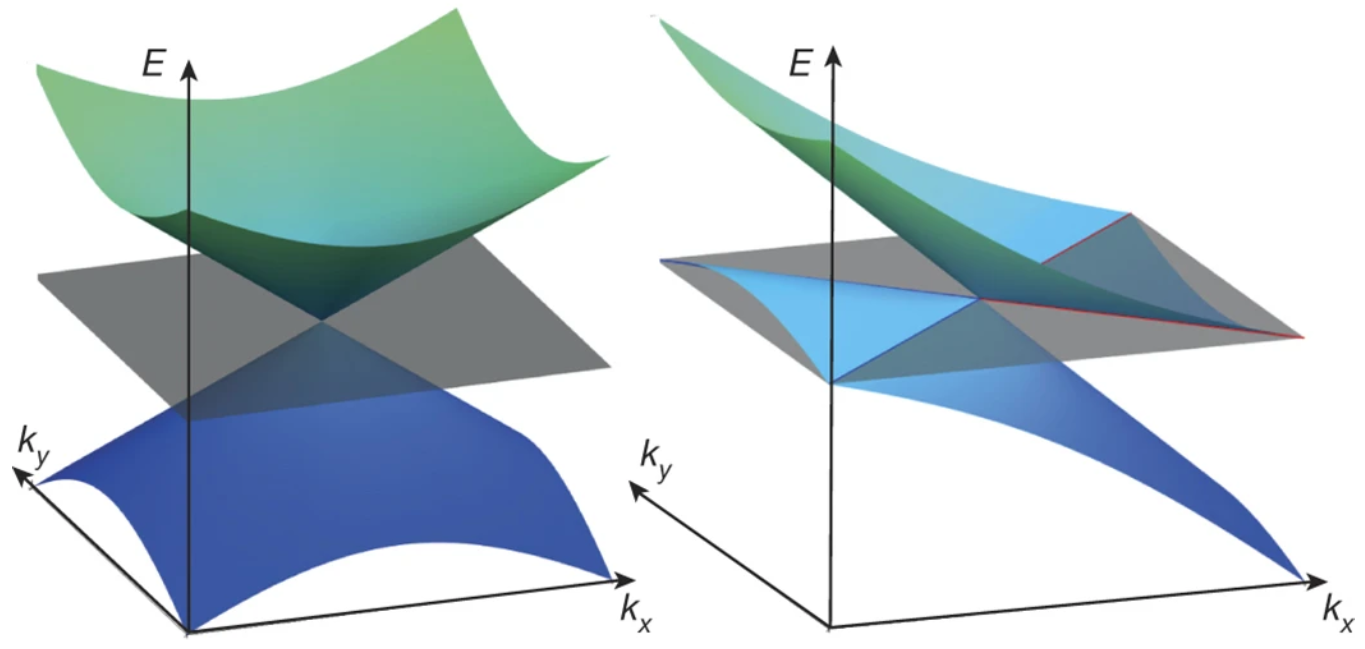
\includegraphics[width=.7\linewidth]{Images/Weyl-cone-tilt}
	\caption{Figure from Ref.~\cite{Soluyanov_Type-II}. Left: Weyl cone in a normal (type I) Weyl semimetal. Right: ``Overtilted'' Weyl cone in a type II Weyl semimetal. Electron and hole pockets are outlined in red and blue, respectively.}
	\label{fig:Weyl-cone-tilt}
\end{figure}
This tipping of the Weyl cone induces significantly altered dispersion, leading to different electronic properties. Such materials are categorised separately as so-called \emph{type II} Weyl semimetals. This distinction is purely physical, however; the different types of Weyl semimetals cannot be distinguished topologically.

\subsection{Nielsen--Ninomiya charge cancellation}

%TODO NN

\subsection{Fermi arcs}

%TODO arcs

\subsection{Semimetals with symmetries}

Thus far, we have discussed Weyl semimetals without assuming any additional symmetry constraints. However, real crystalline solids often naturally possess symmetries beyond simple translational symmetry. Two such symmetries which are especially relevant to the discussion of Weyl semimetals are time-reversal symmetry and inversion symmetry.

%TODO inversion

%TODO time-reversal

%TODO why must one be broken

{\color{blue}
\begin{itemize}
	\item Nielsen--Ninomiya (Chiral anomaly cancelling?)
	
	\item Fermi arcs
	
	\item Discuss the role of inversion + time-reversal symmetry (why one of the two needs to be broken). Topologically different: minimum of 2 vs. 4 Weyl nodes.
	
	\item (Non-linear electric field current response)
\end{itemize}
}


\section{Topological description}\label{sec:semimetal-topology}

%TODO introductory paragraph, give proper credit to Mathai & Thiang

{\color{blue}
\begin{itemize}
	\item Intro paragraph, credit Mathai \& Thiang \cite{Mathai_math-review,Mathai_math-paper}
\end{itemize}
}

\subsection{3D Chern insulators}

To get a good intuition for the topological description of Weyl semimetals, it is useful to first consider a fully insulating material with similar properties. Suppose we have a three-dimensional material that is not subject to any additional symmetries. Such a material is called a 3D Chern insulator, in analogy to the 2D Chern insulator studied in Section~\ref{sec:Chern} \cite{Vanderbilt_2018,Liu_photonic-Chern-vector,Devescovi_3D-Chern}. This system is not a semimetal, but it provides the relevant topological backdrop: Weyl semimetals can be obtained by letting the bands touch in a 3D Chern insulator. As we will discuss shortly, this allows them to act as transitional phases between different insulating topological states.

From the Atland--Zirnbauer classification in Table~\red{[reference]}, %TODO ref. to tenfold way table
one might expect a 3D Chern insulator to be topologically trivial. However, as seen before in Equation~\red{[reference] (and perhaps also in 3D BHZ/Kane--Mele if I discuss this in ch. 2)}, %TODO ref. to weak topology equation
the full topological classification of materials depends not only on the top-dimensional topology, but also on that borrowed from lower-dimensional subspaces. In the case of a 3D Chern insulator, this topology arises on two-dimensional slices of the Brillouin zone; an example of such a slice is highlighted in Figure~\ref{fig:3D_Chern_insulator}.
\begin{figure}[htb!]
	\centering
	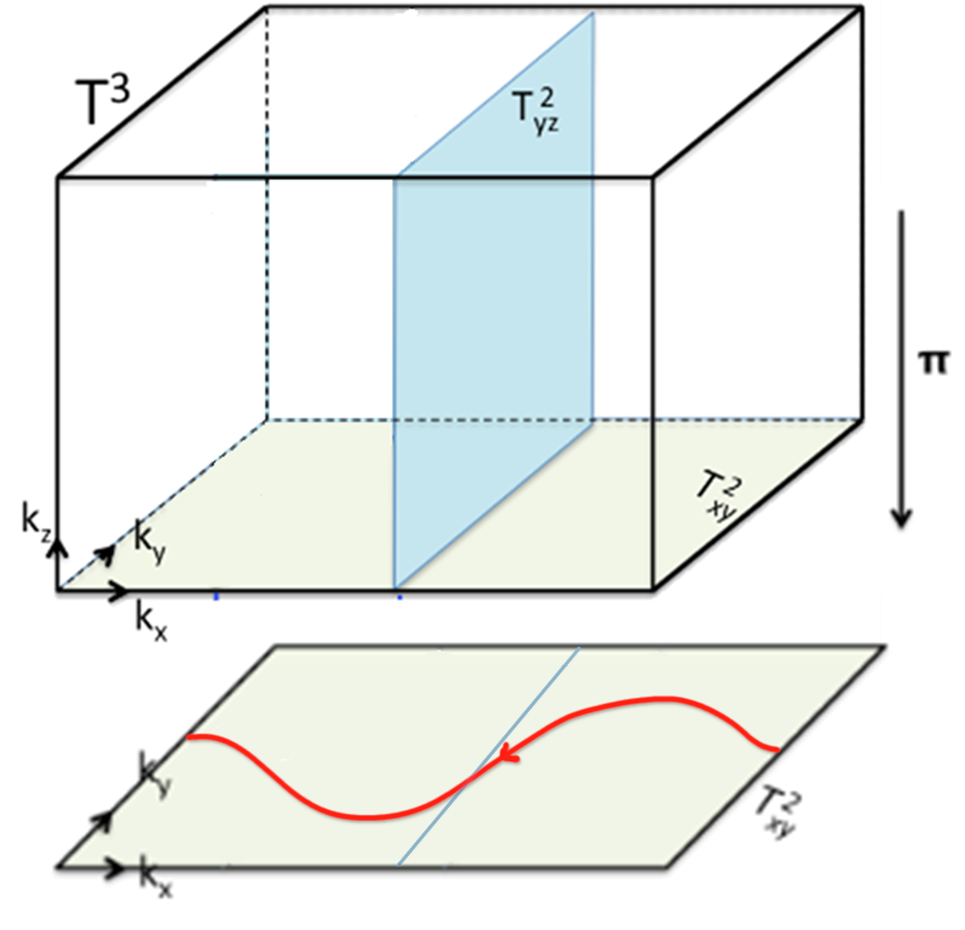
\includegraphics[width=.5\linewidth]{Images/3D_Chern_insulator}
	\caption{Figure adapted from Ref.~\cite{Mathai_math-review}. The three-dimensional Brillouin torus $\T^3$ of a Chern insulator is shown, with a two-dimensional slice $\T_{yz}^2$ indicated in blue. A projection onto a surface Brillouin zone in the $xy$-direction is also shown, with an example Fermi loop of gapless states in red. In this example, the slice $\T_{yz}^2$ has a Chern number of $C_{x} = 1$. Hence, its projection onto the surface is a 1D loop (blue line) that features one chiral band crossing.}
	\label{fig:3D_Chern_insulator}
\end{figure}

There are three topologically distinct ways to slice up the three-torus, all perpendicular to one of the three coordinate directions.\footnote{
	Other 2D slices exist, such as those going diagonally across, but these can all be considered linear combinations of the three ``orthogonal'' slices. To be precise, the different classes of 2D subspaces of $\T^3$ form the second homology group $H_2(\T^3)\cong\Z^3$, and this group is \emph{generated} by the orthogonal slices.}
These slices have the topology of a two-torus $\T^2$, and a Chern number can be obtained by integrating the Berry curvature $\Fc$ of the system over them: for example, perpendicular to the $x$ direction there is a Chern number\footnote{
	Note that it does not matter where along the Brillouin zone the $yz$-slice $\T_{yz}^2$ is taken: the Chern number is an integer, while the system is continuous. This means the $x$ coordinate can be changed continuously without changing the resulting Chern number.}
\begin{equation*}
	C_{x} = \frac{1}{2\pi}\int_{\T_{yz}^2}\!\Fc.
\end{equation*}
This results in a classification by three distinct Chern numbers $C_x$, $C_y$ and $C_z$, which are commonly arranged in a so-called \emph{Chern vector}
\[
	\vb{C} = \begin{pmatrix}
		C_x \\ C_y \\ C_z
	\end{pmatrix} \in \Z^3.
\]

Importantly, these three Chern numbers are all induced by a single two-form $\Fc$. In this sense, there is an exact correspondence between topologically distinct Berry curvatures $\Fc$ and Chern vectors $\vb{C}\in\Z^3$. This is precisely what motivates the use of cohomology for classification: just like in the 2D Chern insulator, the two-form $\Fc$ can be considered to represent a class in the second cohomology group,\footnote{
	As explained in Appendix \ref{chap:homology}, $\Fc$ more properly represents a class in the real-valued \emph{de Rham cohomology} group $H_{\rm dR}^2(\T^3)\cong\R^3$. The analogy is strong enough to be considered direct here, but de Rham cohomology is too plain to encode features such as $\Z_2$ invariants. This is why we elect to use the richer integer-valued cohomology theory.} %TODO perhaps move to ch.2
\begin{equation}\label{eq:2nd-cohom-t3}
	[\Fc]\in H^2(\T^3)\cong\Z^3. 
\end{equation}
As a result, this group precisely classifies the distinct topological phases of the system.\footnote{
	More fundamentally, a complex vector bundle called the \emph{valence bundle} can be associated to a gapped Hamiltonian, and the second cohomology group classifies the different complex vector bundles over a manifold.} %TODO maybe move this to ch.2

\subsubsection{Boundary states}

Before moving on to a system with Weyl points, it will be instructive to study the gapless modes that arise on the surface of a 3D Chern insulator with non-zero Chern vector. Figure~\ref{fig:3D_Chern_insulator} illustrates the case where $\vb{C} = (1,0,0)\tran$. In this case, $\T_{yz}^2$ is the only orthogonal slice with a non-zero Chern number, and as such the material lattice can be thought of as a stack of 2D Chern insulators spanning the $y$ and $z$ directions, stacked together in the $x$ direction. $\T_{yz}^2$ can effectively be considered the Brillouin zone of such a 2D Chern insulator.

Recall from our discussion in Section \ref{sec:Chern} that a 2D Chern insulator with a Chern number of 1 has a single chiral edge mode, which manifests as a gapless state on the one-dimensional surface Brillouin zone. This logic can be translated to the the three-dimensional case, where such slices are stacked in the $x$ direction. Suppose there is a projection $\pi$ along the $z$ direction, onto a two-dimensional surface Brillouin zone $\ext{\T}_{xy}^2$. Then the two-dimensional slices $\T_{yz}^2$ project down to a one-dimensional loop $\pi(\T_{yz}^2)\cong S^1$ containing a single point-like gapless state. As the $\T_{yz}^2$ slice is moved around in the $x$ direction, this band crossing point moves continuously along the $y$ direction, by continuity of the Hamiltonian. It follows that the full two-dimensional surface Brillouin zone must contain a loop of gapless states going across the $x$ direction, as depicted in the figure. This loop is called a \emph{Fermi loop}, in analogy with the Fermi arcs in a Weyl semimetal . Moreover, the chirality of the edge modes can be used to assign a consistent orientation to this loop. %TODO note about linked loops, extra topology etc? Might be unnecessary

Fermi loops admit a natural topological description in terms of homology. Being oriented loops, they precisely represent a class in the first homology group $H_1(\ext{\T}^2)$ of the surface Brillouin zone. Furthermore, it is possible to define an oriented \emph{Dirac loop} $\ell$ in the bulk Brillouin zone in such a way that its projection $\pi(\ell)$ onto the surface in any direction is exactly the Fermi loop. This loop $\ell$ is not a gapless feature,\footnote{
	Dirac loops do still admit a physical interpretation: they represent points at which the Berry connection $\Ac$ has a gauge singularity. Such singularities depend on the choice of gauge, meaning the loop can be moved around by gauge transformations; however, this does not change their topology. The same goes for the Dirac strings that will be discussed in a moment.}
but it is rather interesting topologically: it represents a first homology class in the bulk Brillouin zone,
\[
	[\ell]\in H_1(\T^3)\cong\Z^3.
\]

It is not a coincidence that this first homology group is isomorphic to the second cohomology group $H^2(\T^3)$ from Equation~\eqref{eq:2nd-cohom-t3}. This equivalence is a result of \emph{Poincar\'e duality}, which is the statement that for any closed oriented $d$-dimensional manifold $M$, the isomorphism
\[
	H_n(M) \cong H^{d-n}(M)
\]
holds for any integer $n$. In the present case, this duality can be stated intuitively in terms of Chern numbers, which count the number of signed intersections of the Dirac loop with the different two-dimensional slices of the Brillouin zone.\footnote{
	In general, it is possible that a single Dirac loop ``folds back on itself'' and intersects such a slice more than once. However, any additional intersections introduced in this way always come in oppositely-oriented pairs, leaving the topology unchanged.}
This duality can be summarised schematically as follows:
\begin{equation}\label{eq:duality-scheme}
	H^2(\T^3) \ni [\Fc] \overset{\rm integration}{\iff}
	\vb{C} \overset{\rm intersections}{\iff} [\ell] \in H_1(\T^3).
\end{equation}
This Poincar\'e duality ensures that the classifications in terms of first homology and second cohomology are completely equivalent in this case. Importantly, however, Poincar\'e duality depends on orientability, and it will not hold when we consider non-orientable Brillouin zones in the next chapter. As such, the question of which group provides the right classification of such a system will be key. For the moment, we turn our attention to the topology of Weyl points in the simpler orientable setting.


\subsection{Introducing Weyl points}\label{sec:Weyl-point-topology}

Consider a Weyl semimetal with a set of $k$ Weyl points
\[
	W \equiv \set{w_1,w_2,\ldots,w_k}\subset \T^3.
\]
Then the charge of a Weyl point $w_i$ is given by the Chern number
\begin{equation*}
	C_w = \frac{1}{2\pi}\int_{S_w^2}\!\Fc,
\end{equation*}
where $S_w^2$ is a sufficiently small 2-sphere centred at $w$---in particular, it must be small enough to contain no other Weyl points in its interior. Naively, this might lead us to expect that a semimetal phase is classified by the second cohomology group of the collection of all these spheres:
\begin{equation}\label{eq:2nd-cohom-spheres}
	H^2\left(\bigcup_{i=1}^k S_{w_i}^2\right)\cong \bigoplus_{i=1}^k H^2(S_{w_i}^2) \cong \Z^k.
\end{equation}
However, this classification runs into two problems: it ignores the global cancellation of charge, and it also ignores the additional topology on two-dimensional slices discussed in the previous subsection. Both of these issues are due to the fact that this group only captures the \emph{local} topology near each Weyl point, and they can be addressed by studying how the different Chern numbers on the Brillouin zone must relate to each other \emph{globally}.

The Nielsen--Ninomiya charge cancellation theorem is one such global relation. It is the statement that all the Chern numbers on these 2-spheres must add to zero:
\begin{equation}\label{eq:Nielsen-Ninomiya}
	\sum_{i=1}^{k}C_{w_i} = 0.
\end{equation}
This cancellation can be demonstrated using Stokes' theorem. The argument goes as follows: imagine that the interior of each sphere $S_{w_i}^2$ (i.e.\ a small open 3-ball centred at $w_i$) is removed from $\T^3$. The resulting 3-manifold $X$ looks like a 3-torus with $k$ small ball-shaped holes, and its boundary is given by the collection of spheres:
\[
	\partial X = -\bigcup_{i=1}^k S_{w_i}^2,
\]
where the minus sign induces the correct orientation. Then Stokes' theorem gives
\[
	0 = \frac{1}{2\pi}\int_{\partial X} \dd{\Fc} = -\sum_{i=1}^{k}\frac{1}{2\pi}\int_{S_{w_i}^2}\!\!\Fc = -\sum_{i=1}^{k}C_{w_i},
\]
which is precisely the Nielsen--Ninomiya theorem.

A similar argument can also be applied to study what happens to Chern numbers on two-dimensional slices of the Brillouin zone in this context. This argument is illustrated in Figure~\ref{fig:Weyl-point-Stokes}.
\begin{figure}[htb!]
	\centering
	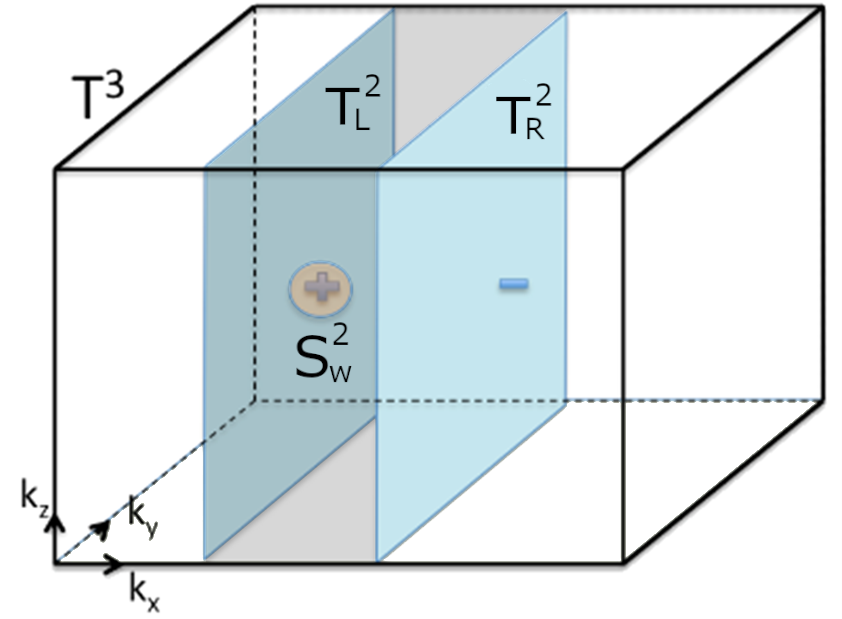
\includegraphics[width=.5\linewidth]{Images/Weyl-point-Stokes}
	\caption{
		Brillouin torus $\T^3$ of a Weyl semimetal with two oppositely charged Weyl points labelled $+$ and $-$. Three two-dimensional subspaces are indicated in blue: a $yz$-like 2-torus on either side of the $+$ point, and a small 2-sphere surrounding it. Given the proper orientation, the blue spaces form the boundary of a three-dimensional manifold $Y$, shaded in grey here.
		Figure from Ref.~\cite{Mathai_math-review}. \red{[not yet licensed; may need better labelling]}%TODO rights, labelling
	}
	\label{fig:Weyl-point-Stokes}
\end{figure}
Here two slices $\T_L^2$ and $\T_R^2$ are placed on either side of a Weyl point $w$ with charge $C_w = q$, along with a small sphere $S_w^2$ surrounding it. These spaces then bound a three-dimensional manifold $Y$ as indicated in the figure, given the following orientations:
\[
	\partial Y = \T_R^2 - \T_L^2 - S_w^2.
\]
The same Stokes' theorem argument can then be used to relate the Chern numbers $C_L$ and $C_R$ on the respective slices, yielding
\[
	C_R = C_L + C_w = C_L + q.
\]
That is, the Chern number of a two-dimensional slice increases by $q$ every time it passes over a Weyl point with charge $q$. As a sanity check, it should be noted that this process respects the periodicity of the Brillouin torus: when the slice is passed over the entire torus, charge cancellation ensures that the added Chern number is zero in total.

All in all, the presence of Weyl points allows for a finer collection of Chern numbers to appear in the Brillouin zone, beyond the $\Z^3$ Chern vector of the insulating case. This behaviour can be captured using cohomology. The key idea is that the Berry curvature has a singularity at points where the gap closes.\footnote{
	Note that this singularity is required in order for the Chern number to change suddenly when a slice (i.e.\ the integration domain of $\Fc$) is moved over a Weyl point continuously.}
As such, it can only be integrated over subspaces where the gap never closes, so that the set of Weyl points $W$ needs to be excluded. This means $\Fc$ now lives in the second cohomology group of the Brillouin zone minus $W$:
\begin{equation}\label{eq:2nd-cohom-semimetal}
	[\Fc]\in H^2\big(\T^3\setminus W\big) \cong \Z^3\oplus\Z^{k-1},
\end{equation}
where $k$ again is the number of Weyl points. Put differently, classification of semimetallic phases given a set of Weyl points $W$ essentially amounts to classifying the gapped phases on the punctured torus $\T^3\setminus W$.

Notably, this classification addresses both issues present in the $\Z^k$ classification on 2-spheres in Equation~\eqref{eq:2nd-cohom-spheres}. Firstly, it incorporates 3D Chern insulator topology in the first term, in the form of the $\Z^3$ from Equation~\eqref{eq:2nd-cohom-t3}. Perhaps more subtly, charge cancellation is also incorporated in the form of the reduction by one $\Z$ factor in the second term. This can be understood intuitively: for example, if $k=1$ then the Nielsen--Ninomiya theorem implies that the single Weyl point must have a charge of 0, and so it is not topologically protected. A similar intuition holds for larger $k$, in that the $k$ additional ``degrees of freedom'' which are afforded to the system by the Weyl point charges are reduced by one under the charge cancellation condition. This relation will become more explicit once the Mayer--Vietoris sequence is introduced in Section \ref{sec:Mayer-Vietoris}.

%Notably, there are $k-1$ extra factors of $\Z$ involved in the classification of a Weyl semimetal compared to that of a 3D Chern insulator (cf.\ Equation~\eqref{eq:2nd-cohom-t3}). This contrasts with the $k$ factors found for the collection of spheres in Equation~\eqref{eqeq:2nd-cohom-spheres}. This reduction by one is a natural result of charge cancellation: for example, if $k=1$ then the Nielsen--Ninomiya theorem implies that the single Weyl point must have a charge of 0, and so it is not topologically protected. A similar intuition holds for general $k\in\N$, in that the $k$ additional ``degrees of freedom'' which are afforded to the system by the Weyl point charges are reduced by one under the charge cancellation condition. This relation will become more explicit once the Mayer--Vietoris sequence is introduced in Section \ref{sec:Mayer-Vietoris}.


\subsubsection{Fermi arcs}

The varying Chern numbers over Weyl points help explain how Fermi arcs arise on the surface. As discussed in the case of a 3D Chern insulator, Fermi loops on the surface arise whenever there is a non-zero Chern number in some direction. Similarly, Fermi arcs begin and terminate whenever the presence of a Weyl point causes a change in the Chern number; this is illustrated in Figure~\ref{fig:Fermi-arc-Chern}.
\begin{figure}[htb!]
	\centering
	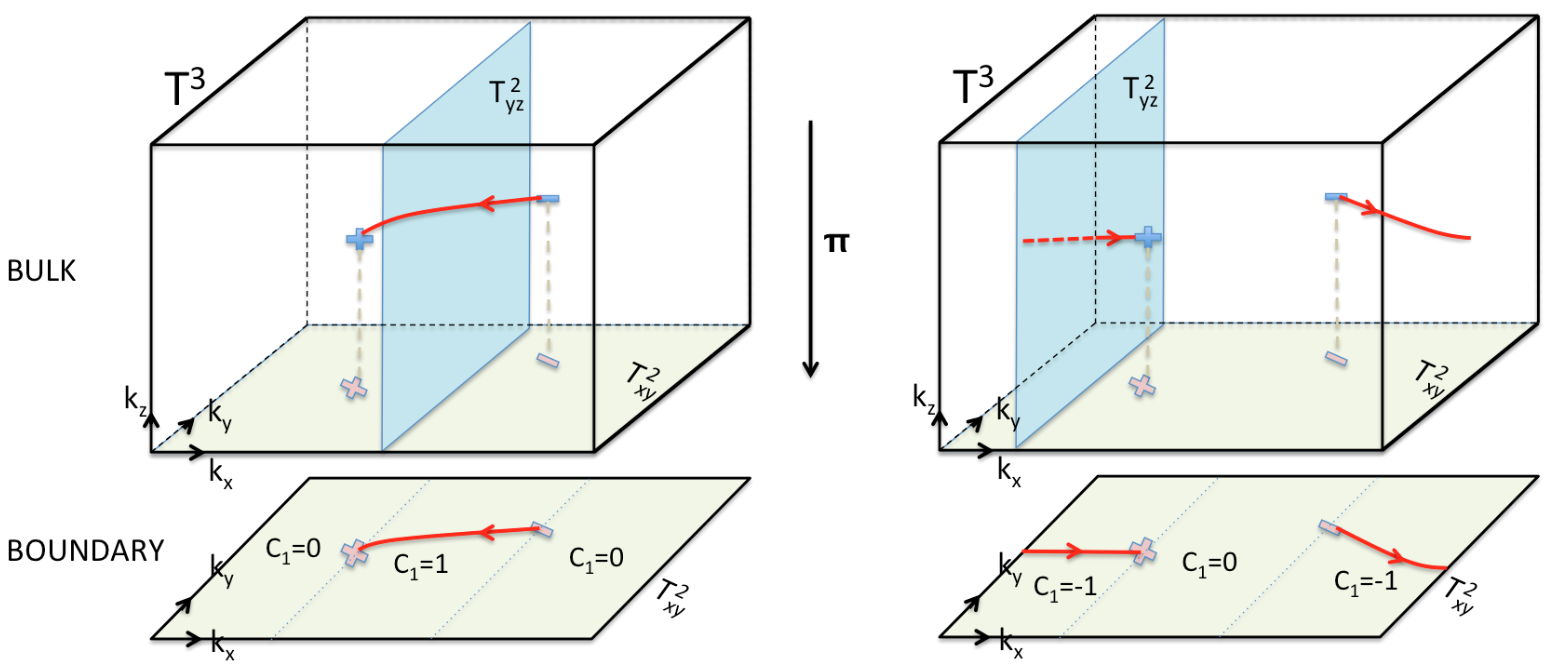
\includegraphics[width=\linewidth]{Images/Fermi-arc-Chern}
	\caption{
		Two semimetal Brillouin zones are shown with the same configuration of Weyl points, but featuring topologically distinct Fermi arcs (shown in red on the boundary). The distinction is due to different bulk Chern numbers: Fermi arcs appear in regions where the bulk Chern number is non-zero. These Fermi arcs can be considered to be the projection of a Dirac string (shown in red in the bulk).
		Figure from Ref.~\cite{Mathai_math-review}.}
	\label{fig:Fermi-arc-Chern}
\end{figure}

This feature of Weyl semimetals implies they can mediate phase transitions between 3D Chern insulators with different Chern vectors. For example, suppose a pair of Weyl points is created at some point in the Brillouin zone of a trivial insulator ($\vb{C}=0$). These points can then be moved apart in the $z$ direction until they meet again and annihilate at the other end of the torus. In the process, a Fermi arc extends between the projections of the Weyl points on the $xz$ and $yz$-planes, which eventually closes into a Fermi loop. In its final state, the system features a non-zero Chern vector of $\vb{C} = (0,0,1)\tran$.

This process was first observed experimentally in a seminal work by Gui-Geng Liu et al.\ in 2022. The authors construct a photonic crystal, which is a type of artificial crystal where the different energy levels are represented by frequencies of light. Under application of a magnetic field, this crystal undergoes a transition between trivial and topological insulating phases, mediated by the creation and annihilation of two Weyl points; see Figure~\ref{fig:Weyl-phase-transition}.
\begin{figure}[htb!]
	\centering
	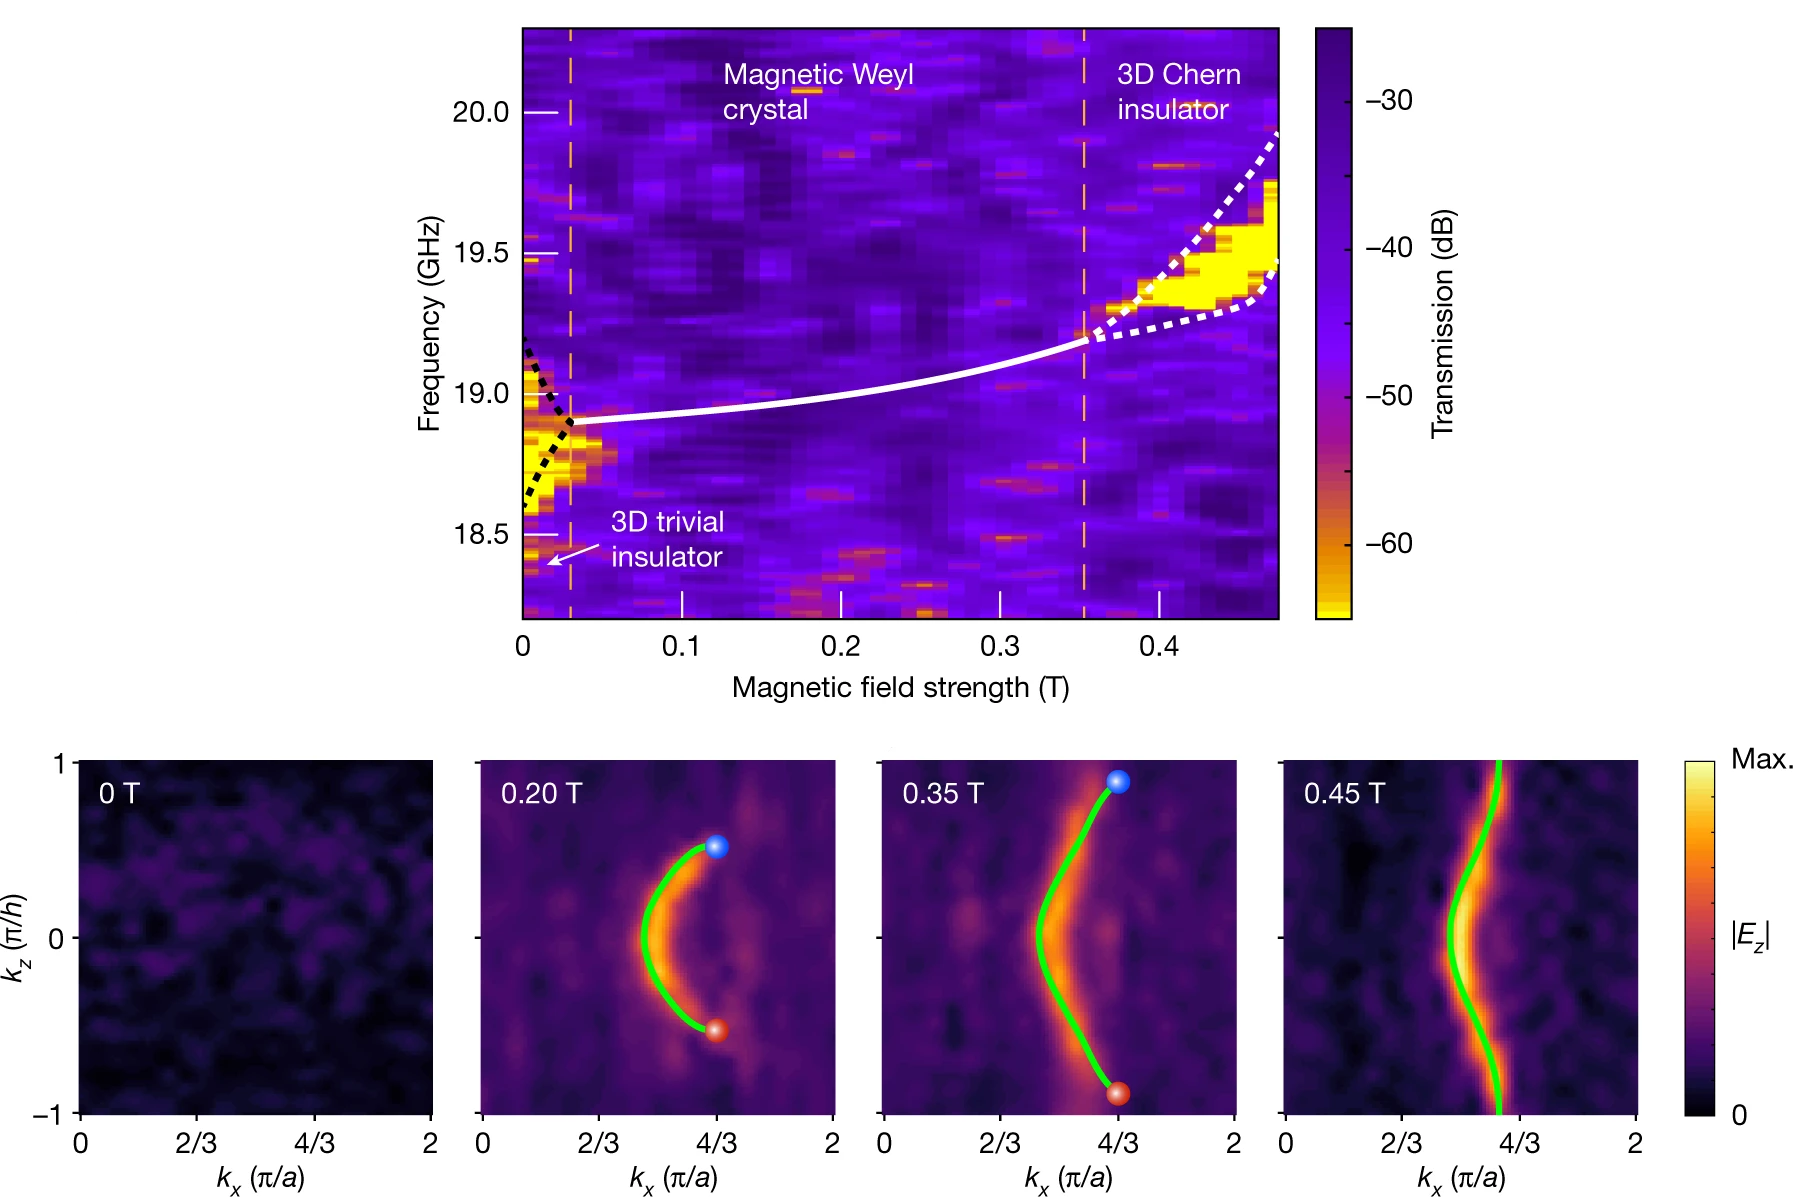
\includegraphics[width=\linewidth]{Images/Weyl-phase-transition}
	\caption{Figure from Ref.~\cite{Liu_photonic-Chern-vector}, reproduced with permission from Springer Nature.
		Top: measured frequency response (i.e.\ ``band structure'') at increasing magnetic field strength. Yellow regions represent a band gap in the spectrum, indicating insulating phases. The white line represents the calculated frequency of the two Weyl nodes in the system. Bottom: measured response on a surface Brillouin zone, at the frequencies indicated on the white line above. Simulated Fermi arcs and loops are shown in green. A Fermi loop can clearly be seen to form, confirming a phase change to a topological insulator.}
	\label{fig:Weyl-phase-transition}
\end{figure}
This was also the first experimental realisation of a 3D Chern insulator \cite{Liu_photonic-Chern-vector}, and of a system featuring a single Fermi arc.

Just as Fermi loops can be considered projections of a bulk Dirac loop, so too can Fermi arcs be considered a projection of a bulk \emph{Dirac string}.\footnote{
	A more or less equivalent concept is referred to as \emph{Euler chain} in \cite{Mathai_math-review}, placing the emphasis on topology over physics: ``chain'' here refers the oriented subspaces that homology is founded on.}
Like Dirac loops, these strings can be given an interpretation in terms of homology. The setup is somewhat more subtle in this case: since the Dirac strings have a boundary, they are not loops and as such do not represent homology classes in $H_1(\T^3)$. Instead, they represent classes in the \emph{relative homology group}
\begin{equation}\label{eq:relative-homology}
	H_1\big(\T^3, W\big) \cong \Z^3\oplus\Z^{k-1}
\end{equation}
with respect to the set of Weyl points $W\subset\T^3$. Intuitively, taking the relative homology means that any boundaries lying in the subset $W$ are ignored; for a more precise definition the reader is referred to \parencite[\S 2.1]{Hatcher_algebraic-topology}.

This homology picture provides a classification scheme that is exactly dual to the cohomology classification in Equation~\eqref{eq:2nd-cohom-semimetal}; that is, there is an isomorphism
\begin{equation}\label{eq:semimetal-duality}
	H^2\big(\T^3\setminus W\big) \cong H_1\big(\T^3, W\big).
\end{equation}
This is not a direct Poincar\'e duality, but it is nevertheless mathematically rigorous and protected by orientability in the same way.\footnote{
	To be precise, Poincar\'e duality does not hold directly because $\T^3\setminus W$ is not a closed manifold. Instead, for non-compact manifolds $M$ there is a generalized duality $H^n(M)\cong H_{d-n}^{\rm BM}(M)$ where the group on the right is the \emph{Borel--Moore homology}, and this is in turn equivalent to the relative homology in this case. Alternatively, Equation~\eqref{eq:semimetal-duality} can be interpreted as a result of the so-called \emph{Lefschetz duality} $H^n(M)\cong H_{d-n}(M, \partial M)$ for manifolds with a boundary.}
The interpretation in terms of Chern numbers given in Equation~\eqref{eq:duality-scheme} also still holds here, with the Chern vector and Dirac loops replaced with more general Chern numbers and Dirac strings, respectively.


\subsection{The semimetal Mayer--Vietoris sequence}\label{sec:Mayer-Vietoris}

In the previous section a heuristic Stokes' theorem argument was discussed for charge cancellation on Weyl points. This argument can be generalized by moving to a more abstract cohomology setting, where we are not dependent on the integration of forms; this is important because integration will not be well defined once we move to a non-orientable setting. As an added bonus, the abstract description proves to be richer and provide more detailed information on the possible topological phases for a Weyl semimetal.

The idea is that the relation between the global semimetal topology in Equation~\eqref{eq:2nd-cohom-semimetal} and the local charge data in Equation~\eqref{eq:2nd-cohom-spheres} can be understood by considering how cohomology classes are mapped between them. That is, one needs to find and study a homomorphism
\begin{equation*}
	\beta: H^2\big(\T^3\setminus W\big) \to H^2\left(\bigcup_{i=1}^k S_{w_i}^2\right).
\end{equation*}
Such a map arises naturally in the context of the \emph{Mayer--Vietoris sequence} for cohomology.

Mayer--Vietoris sequences are used to study how the homology or cohomology of a topological space relates to that of its subspaces. To be precise, let $X$ be a topological space and let $A,B\subset X$ be two subspaces that cover it (i.e.\ $A\cup B = X$). Then there is an \emph{exact sequence} of homomorphisms between cohomology groups,
\begin{equation*}
	\cdots \to H^n(X) \to H^n(A)\oplus H^n(B) \to H^n(A\cup B) \to H^{n+1}(X) \to \cdots,
\end{equation*}
which continues indefinitely in both directions. Exactness means that the image of each map in the sequence is exactly equal to the kernel of the next. In other words, the elements in each term in the sequence which are mapped to zero in the next term are precisely those which ``descend'' from the previous term. In particular, the composition of two subsequent maps always yields zero.

In the context of a Weyl semimetal there is a natural way to divide the Brillouin torus $\T^3$ into two subspaces; this is illustrated in Figure~\ref{fig:semimetal-MV}.
\begin{figure}[htb!]
	\centering
	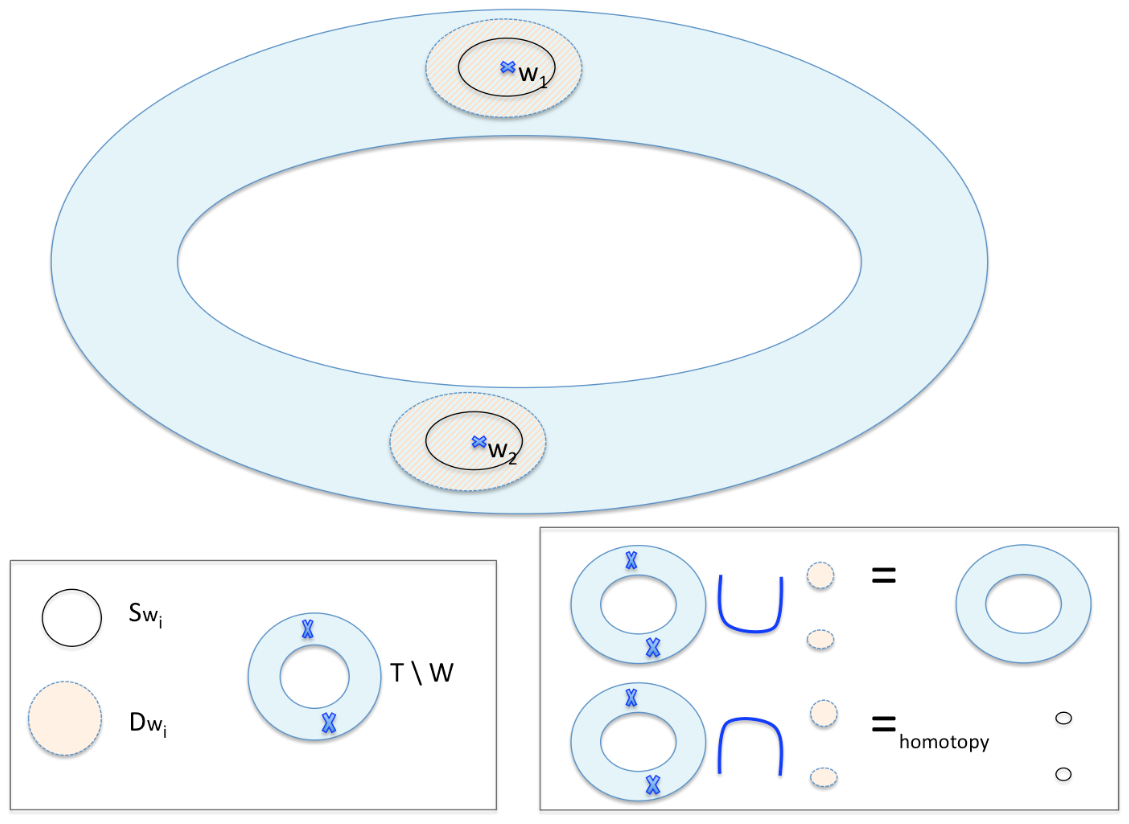
\includegraphics[width=.8\linewidth]{Images/semimetal-MV}
	\caption{
		Schematic two-dimensional representation of the Brillouin torus and the subspaces used to cover it.
		Figure from Ref.~\cite{Thiang_equivariant}}
	\label{fig:semimetal-MV}
\end{figure}
The first subspace in the covering is the punctured torus $\T^3\setminus W$; we have already encountered this space in classifying topological semimetal phases. The other is the collection $\bigcup_{i=1}^k D_{w_i}^3$ of small open 3-balls centred on the Weyl points $w_i$. The intersection of these two spaces is the same collection of open balls, but each with a single puncture. For our purposes, this intersection has the same topology as the collection of 2-spheres $\bigcup_{i=1}^k S_{w_i}^2$ that we encountered in the context of local Weyl point charges.\footnote{
	To be precise, the punctured 3-balls can be \emph{deformation retracted} into the 2-spheres, making them \emph{homotopy equivalent}. Homotopy equivalent spaces have the same homology and cohomology groups.}
A Mayer--Vietoris sequence can now be written down for these subspaces. The section of this sequence which is relevant to classification is referred to as the \emph{semimetal Mayer--Vietoris sequence}:\footnote{
	Note that the open balls $D_{w_i}^3$ do not appear in this sequence at all. This is because they can be contracted to a point, and hence are topologically trivial in a sense.}
\begin{equation}\label{eq:semimetal-MV-symbolic}
	0\ \to\ \underbrace{H^2(\T^3)}_{\mathclap{\text{3D Chern insulator}}}\ \to\ 
	\underbrace{H^2\big(\T^3\setminus W\big)}_{\text{Semimetal}}\ \overset{\beta}{\to}\ \underbrace{H^2\!\left(\bigcup_{i=1}^k S_{w_i}^2\right)}_{\text{Local charges}}\ \overset{\Sigma}{\to}\ H^3(\T^3)\ \to\ 0.
\end{equation}
The first three groups in this sequence are already familiar from Equations \eqref{eq:2nd-cohom-t3}, \eqref{eq:2nd-cohom-semimetal} and \eqref{eq:2nd-cohom-spheres} respectively. The last group $H^3(\T^3)\cong\Z$ is represented by volume forms\footnote{
	I.e.\ 3-forms, which are locally proportional to $\dd{k_x}\wedge\dd{k_y}\wedge\dd{k_z}$.}
on the torus; one notable example of such a form is the trivial 3-form
\begin{equation*}
	\dd{\Fc} = 0 \in H^3(\T^3)
\end{equation*}
which appeared in the Stokes' theorem arguments previously. Indeed, the map labelled $\Sigma$ above can be loosely interpreted as the exterior derivative $\dd$. However, a more physically useful interpretation is that $\Sigma$ gives the total charge in the system: it sends a set of Chern numbers on the Weyl points to their sum in $\Z$.

Explicitly, the semimetal Mayer--Vietoris sequence is\footnote{
	In principle the direct sum in the semimetal group has little mathematical significance; we write $\Z^3\oplus\Z^{k-1}$ instead of $\Z^{k+2}$ to aid the physical interpretation.}
\begin{equation}\label{eq:semimetal-MV-explicit}
	0 \to \Z^3 \to \Z^3\oplus\Z^{k-1} \overset{\beta}{\to} \Z^k \overset{\Sigma}{\to} \Z \to 0.
\end{equation}
The exactness of this sequence can be used to extract useful information, especially around the group of local charges $\Z^k$. Here exactness means that $\im(\beta) = \ker(\Sigma)$. This implies that the local charges on the Weyl points sum to zero if and only if they descend from a semimetal. In other words, it implies not only the Nielsen--Ninomiya charge cancellation theorem, but also its converse: any set of Weyl points with charges adding to zero is admissible as a topological Weyl semimetal phase.

In fact, more can be inferred by looking at the maps around the semimetal group $\Z^3\oplus\Z^{k-1}$. Here exactness tells us that $\ker(\beta)\cong\Z^3$. This makes physical sense: if all local charges are zero, the Weyl points are not topologically protected and the system is really in a 3D Chern insulator phase. However, since $\beta$ is a homomorphism, we also find $\beta^{-1}(c)\cong\Z^3$ for a generic charge configuration $c\neq 0\in\Z^k$; that is, every configuration with total charge zero admits a $\Z^3$ worth of topologically different semimetal phases. This makes precise a principle that is also hinted at in Figure~\ref{fig:Fermi-arc-Chern}: Weyl semimetals with identical charge configurations may nevertheless be topologically distinct, and their topologies differ by a bulk Chern vector in $\Z^3$.\footnote{
	Properly speaking, the set of topological phases for a given charge configuration is an affine space for $H^2(\T^3)$, since there is no canonical zero Chern vector on a Weyl semimetal. This is worked out in greater mathematical detail in Section 3 of \cite{Mathai_math-review}.}


\subsubsection{The dual homology sequence}

In previous subsections, we have already seen that the cohomology invariants on Chern insulators and Weyl semimetals can be understood equally well in terms of homology groups. As it turns out, this duality can be extended to the semimetal Mayer--Vietoris sequence \eqref{eq:semimetal-MV-symbolic}. The dual of the first two groups was already explored in Equations \eqref{eq:duality-scheme} and \eqref{eq:semimetal-duality}. The latter two groups act on closed manifolds, and so their dual can be obtained from Poincar\'e duality directly:
\begin{equation*}
	H^2\left(\bigcup_{i=1}^k S_{w_i}^2\right) \cong H_0\left(\bigcup_{i=1}^k S_{w_i}^2\right), \qquad
	H^3(\T^3) \cong H_0(\T^3).
\end{equation*}
In both cases, we have a top-dimensional cohomology group (containing volume forms) being dualised to a zeroth homology group, which counts the number of connected components. In particular, since the connected components are the important aspect, the 2-spheres $S_w$ may be substituted for the Weyl points $w$ to simplify:
\begin{equation*}
	H_0\left(\bigcup_{i=1}^k S_{w_i}^2\right) \cong H_0(W).
\end{equation*}
The complete homology dual of \eqref{eq:semimetal-MV-symbolic} is then
\begin{equation}\label{eq:semimetal-homology-sequence}
	0\ \to\ \underbrace{H_1(\T^3)}_{\mathclap{\text{Dirac loops}}}\ \to\ 
	\underbrace{H_1\big(\T^3, W\big)}_{\text{Dirac strings}}\ \overset{\partial}{\to}\ \underbrace{H_0(W)}_{\mathclap{\text{Local charges}}}\ \overset{\Sigma}{\to}\ H_0(\T^3)\ \to\ 0.
\end{equation}

This exact sequence has arisen through taking Poincaré duals of groups in the Mayer--Vietoris sequence, but somewhat miraculously, it continues to be valid even in the absence of Poincaré duality (e.g.\ on a non-orientable manifold). In fact, it can be considered a more fundamental sequence in some ways: it describes the homology of the torus with respect to a single subspace $W$, whereas the Mayer--Vietoris sequence relies on multiple subspaces that cover the torus.\footnote{
	Indeed, this is the first exact sequence introduced in the standard algebraic topology textbooks, e.g.\ in Theorem 2.13 of \cite{Hatcher_algebraic-topology}.}
	
The map indicated by $\partial$ is the boundary map that is used to define homology groups in the first place.\footnote{
	To be precise, homology is defined using boundaries of chains; one can think of the present map as acting on \emph{representatives} of homology classes.}
In this case, it sends classes of oriented Dirac strings in the bulk to the Weyl points that bound them, with a sign given by which end of the string the points are on. For example, for a Weyl semimetal with two Weyl points $W = \set{w_1,w_2}$ connected by a Dirac string $s$, we have $[s]\in H_1(\T^3,W)$ and
\begin{equation*}
	\partial\big([s]\big) = (1, -1)\in H_0(W)\cong\Z^2. 
\end{equation*}
This gives rise to a very natural interpretation of charge cancellation: it automatically follows from the fact that Weyl points on opposite ends of a Dirac string are assigned opposite signs. These opposite charges are then summed to zero by the total charge map $\Sigma$, i.e.\ $\Sigma\circ\partial = 0$. This can also be inferred from the exactness of \eqref{eq:semimetal-homology-sequence}, which additionally tells us that there exists a configuration of Dirac strings compatible with any set of Weyl points with total charge zero.

As emphasised before, this homology sequence encodes exactly the same information as the cohomology Mayer--Vietoris sequence in the simple case where Poincaré duality is preserved. However, once symmetries are imposed on the system, this duality may be altered, in which case the two basic sequences become essentially different. It then becomes necessary to study how the cohomology and/or homology groups must be altered to encode relevant information about the topological phases of the system. We will review one example of this in the next section.


\subsection{Time-reversal symmetric Weyl semimetals}\label{sec:T-WSMs}

The preceding topological review of Weyl semimetals has thus far been in the context of the basic symmetry class A---that is, we have not imposed any additional symmetries on the system. However, such additional symmetries are not necessarily forbidden in a Weyl semimetal: the type A classification merely tells us that the semimetal topology is very robust, not relying on any symmetry protection.\footnote{
	By contrast, for example, the SSH model introduced in Section~\ref{sec:SSH} has chiral symmetry-protected topological phases.}
As discussed in Section~\ref{sec:semimetal-physics}, either time-reversal symmetry or lattice inversion symmetry needs to be broken in order to realise a Weyl semimetal. In practice, it is often very natural for time-reversal invariance to be preserved in the absence of a magnetic field, and many candidate materials are indeed time-reversal symmetric \cite{Weng_WSM-candidates,Huang_WSM-candidates,Lv_WSM-TaAs,Xu_WSM-experiment,Belopolski_minimal-WSM}. An excellent topological description of such systems was published by Guo Chuan Thiang, Koji Sato and Kiyonori Gomi in 2017, and we will spend the rest of this section reviewing its main aspects \cite{Thiang_equivariant}.

Preserving time-reversal symmetry puts us in class AII of the tenfold way classification in Table~\red{[cite table]}, %TODO tenfold way table
meaning the underlying insulating topology (i.e. the topology with zero Weyl points) is that of the strong and weak insulators described in Section~\ref{sec:3D-Z2}. This means the four $\Z_2$ invariants (three weak and one strong) in such systems also play a role in the semimetal topology. Just as class A Weyl semimetals can be considered intermediate phases between different 3D Chern insulators (as shown in Figure~\ref{fig:Weyl-phase-transition}), it is shown in Ref.~\cite{Thiang_equivariant} that class AII semimetals can mediate phase transitions between different strong and weak 3D insulators via Weyl point creation and annihilation.

As discussed in Section~\ref{sec:semimetal-physics}, time reversal symmetry squaring to $\TRS^2=-1$ forces Weyl points to appear in Kramers pairs of the same chirality, related by $\k\leftrightarrow-\k$ in the Brillouin zone. The topology induced by the presence of these pairs must also respect the symmetry, and as such it cannot be studied by simply moving integration planes freely over the individual Weyl points (as previously shown in Figure~\ref{fig:Weyl-point-Stokes}). Indeed, recall from Section~\ref{sec:3D-Z2} that the insulating $\Z_2$ invariants must be calculated specifically at the $\TRS$-invariant planes sitting at $k_{x,y,z}\in\{0,\pm\pi\}$. To study how Kramers pairs affect these invariants, their respective planes must be continuously deformed across them in a way that respects the symmetry, leading to the concept of \emph{curved $\TRS$-planes}; see Figure~\ref{fig:T-planes}.
\begin{figure}[htb!]
	\centering
	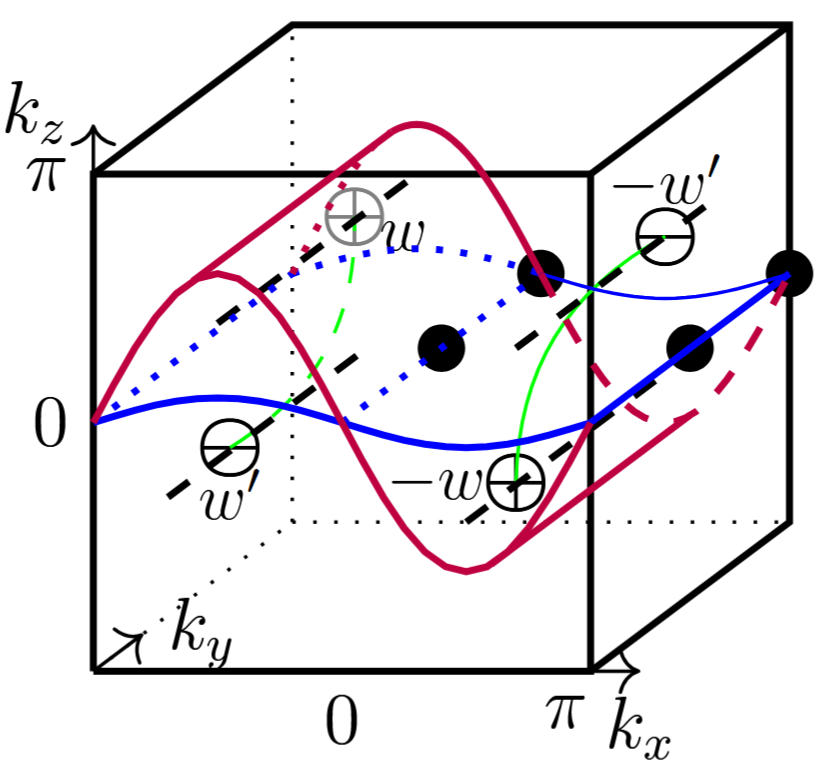
\includegraphics[width=.5\linewidth]{Images/T-planes}
	\caption{Figure from Ref.~\cite{Thiang_equivariant}. Curved $\TRS$-planes are shown in blue and purple; both are deformations of the $k_z=0$ plane. Deforming the blue plane into the purple one makes it cross the Kramers pair at $\k=\pm w$. This induces a change in the related $\Z_2$ invariant: if the Weyl points in this pair have individual charges of $q$, then the invariants on these planes are related by $\Delta_{z,0}^{\rm purple} \equiv \Delta_{z,0}^{\rm blue} + q \mod 2$.} %TODO rights
	\label{fig:T-planes}
\end{figure}

The cohomology description must be altered in several ways in order to accommodate this more complex topology. First of all, the cohomology classes must respect the $\k\leftrightarrow-\k$ symmetry on the Brillouin zone, leading to the use of \emph{equivariant} cohomology groups $H_{\Z_2}^n$, where the $\Z_2$ stands for the $\Z_2$ action of the symmetry. Mathematically, this is similar in spirit to studying the topology of the \emph{effective Brillouin zone} covering half the torus $\T^3$, obtained from the quotient $\T^3/\Z_2$ of the symmetric action. However, the presence of high-symmetry points means some topological information is lost in passing to this effective Brillouin zone, and so a somewhat more involved construction called the \emph{homotopy quotient} must be employed instead.\footnote{
	This homotopy quotient is obtained from the \emph{Borel construction}, relying on the fact that there is always a contractible space $EG$ (the total space of the so-called \emph{universal bundle}, in this case $S^\infty$) on which the symmetry group $G$ acts freely. The product space $EG\times\T^3$ is then homotopy equivalent to $\T^3$, but the diagonal action has no fixed points. Equivariant cohomology is defined as the cohomology of the quotient space of this action: $H_G^n(\T^3) := H^n(EG\times_G\T^3)$.}

Secondly, the non-trivial topology existing at the time-reversal invariant momenta (TRIM) necessitates that the cohomology groups be calculated relative to these points. This relative cohomology is defined in much the same way as the relative \emph{homology} featured in Equation~\eqref{eq:relative-homology}.

Lastly, the cohomology must be \emph{twisted}; that is, it is endowed with \emph{local coefficients} $\ext{\Z}$, which change sign under the $\Z_2$ action of the symmetry. We will provide a more geometric intuition behind these local coefficients in Section~\ref{sec:non-ori_topology}.

All in all, the regular cohomology groups in the Mayer--Vietoris sequence in Equation~\eqref{eq:semimetal-MV-symbolic} must be changed to rather complicated \emph{twisted equivariant} cohomology \emph{relative} to the TRIM. For example, the insulating invariants (i.e.\ Chern vectors) in $H^2(\T^3)\cong\Z^3$ are altered to
\begin{equation*}
	H_{\Z_2}^2(\T^3, \text{TRIM}; \ext{\Z}) \cong \Z_2^4,
\end{equation*}
containing precisely the four $\Z_2$ invariants: three weak and one strong. The use of this form of cohomology is motivated in Ref.~\cite{Thiang_equivariant} by the classification of so-called ``Quaternionic'' vector bundle structures on the Brillouin zone, which are a modification of the usual complex vector bundles induced by the $\TRS^2=-1$ symmetry \cite{NittisGomi_Quaternionic,NittisGomi_FKMM}.

The dual homology picture is considerably simpler in this case. The only modification necessary to the groups in the homology sequence in Equation~\eqref{eq:semimetal-homology-sequence} is the use of equivariant homology $H_n^{\Z_2}$; %TODO on mfd excluding TRIM?
that is, instead of generic Dirac loops and strings, the homology classes must be represented by their \emph{$\TRS$-stable} variants which respect the $\k\leftrightarrow-\k$ symmetry and avoid the TRIM. Just as in the type A system, this leads to an intuitive description of the associated invariants; see for example Figure~\ref{fig:TRS-loops}.
\begin{figure}[htb!]
	\centering
	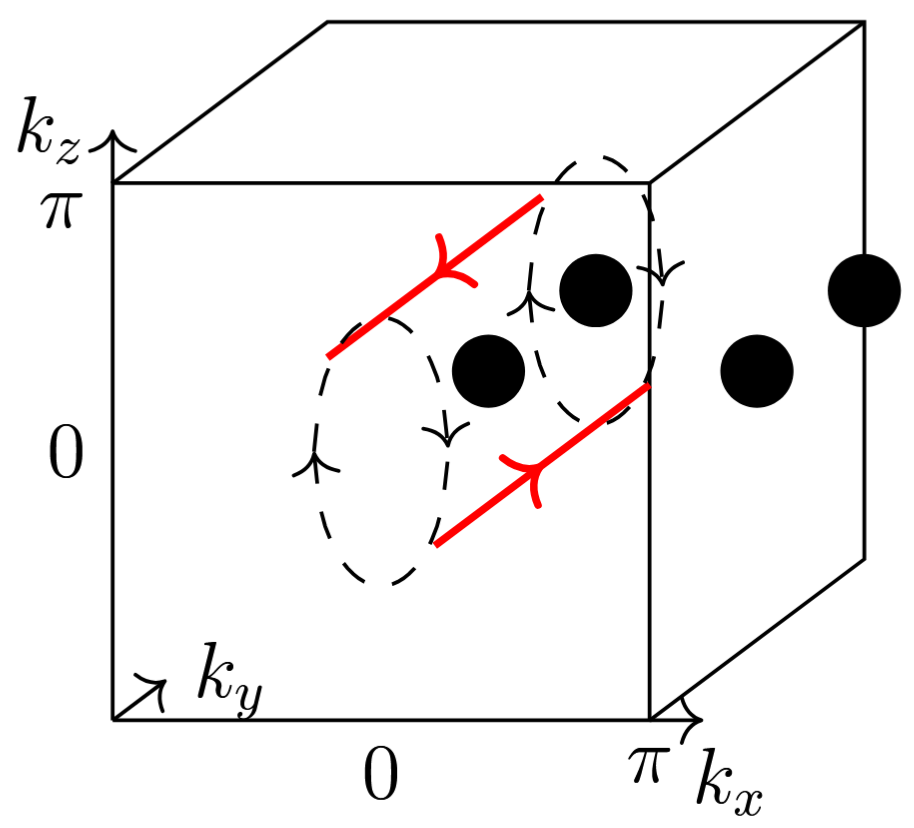
\includegraphics[width=.5\linewidth]{Images/TRS-loops}
	\caption{Figure from Ref.~\cite{Thiang_equivariant}. A $\TRS$-stable pair of oriented Dirac loops $l_y$ is shown spanning the $k_y$ direction. The loops may be interchanged while maintaining $\TRS$-stability, by rotating them along the dashed lines. Doing so recovers the original pair with opposite orientation. It follows that $l_y=-l_y$, that is, $2l_y = 0$; as a result, $l_y$ generates a $\Z_2$ invariant, dual to the cohomology invariant $\nu_y$.} %TODO rights
	\label{fig:TRS-loops}
\end{figure}

Calculated using either homology or cohomology, the semimetal Mayer--Vietoris sequence takes on the following explicit form in a class AII system:
\begin{equation}\label{eq:TRS-MV-explicit}
	0 \to \Z_2^4 \to \Z_2^4\oplus\Z^{r-1} \overset{\beta}{\to} \Z^r \overset{\Sigma}{\to} \Z \to 0,
\end{equation}
where in this case, $r$ labels the number of Kramers pairs rather than individual Weyl points. Its features are very much analogous to the class A sequence in Equation~\eqref{eq:semimetal-MV-explicit}: it is essentially obtained by substituting the $\Z^3$ relating to insulating Chern vectors with a $\Z_2^4$ indexing the weak and strong invariants. Just as before, the map $\Sigma$ can be used to deduce Nielsen--Ninomiya charge cancellation, and the semimetal group $\Z_2^4\oplus\Z^{r-1}$ combines the insulating invariants on the left with a $\Z^{r-1}$ representing the set of allowed Weyl point charge configurations. The main difference from the class A case is that the topology is framed in terms of pairs of Weyl points, and as such the minimum number of Weyl points is four instead of two---as we also covered in the physical setting of Section~\ref{sec:semimetal-physics}.

One might reasonably question whether the classification of Weyl semimetals with additional symmetries always comes down to a mere change in the underlying insulating topology, as it does in this case. In Chapter~\ref{chap:non-orientable}, we will discuss a counterexample to this: we show that the Mayer--Vietoris sequence is altered more radically under a symmetry which has previously been demonstrated to induce novel semimetal topology.
